\documentclass[12pt]{article}
\usepackage{amsmath}  % Math
\usepackage{amssymb}  % Symbols
\usepackage{graphicx} % Images
\usepackage[utf8]{inputenc}
\usepackage[T1]{fontenc}
\usepackage[margin=1in]{geometry}
\usepackage[spanish]{babel}
\usepackage{transparent}
\usepackage{eso-pic}
\usepackage{xcolor}
\usepackage{subcaption} % For subfigures
\usepackage{array} % For thicker table lines and better column definitions
\usepackage{booktabs} % For professional quality tables
\usepackage{longtable} % For tables that span multiple pages
\usepackage{float} % For [H] option in tables/figures

\graphicspath{{images/}} % Path to images
\newcommand\BackgroundPic{
    \put(0,0){
        \parbox[b][\paperheight]{\paperwidth}{
            \vfill
            \centering
            \transparent{0.1}
\includegraphics[width=\paperwidth]{logo} % your image
            \vfill
        }
    }
}


\title{Informe Negocio Empanadas: \\
\textit{Las Empanadas Hermanas}} % Title of the report
  \author{Autores: Felipe Colli, Juan Gonzalez, Bastián Ortiz y Javier Robles \thanks{Instituto Nacional General José Miguel Carrera} \\
  Curso: \textit{4°H}, Profesor: \textit{Carlos Morales}} % Add your names and course
  \date{30 de mayo de 2025} % Fecha de Entrega
\AddToShipoutPicture{\BackgroundPic} % Add background image

\begin{document}

\maketitle
%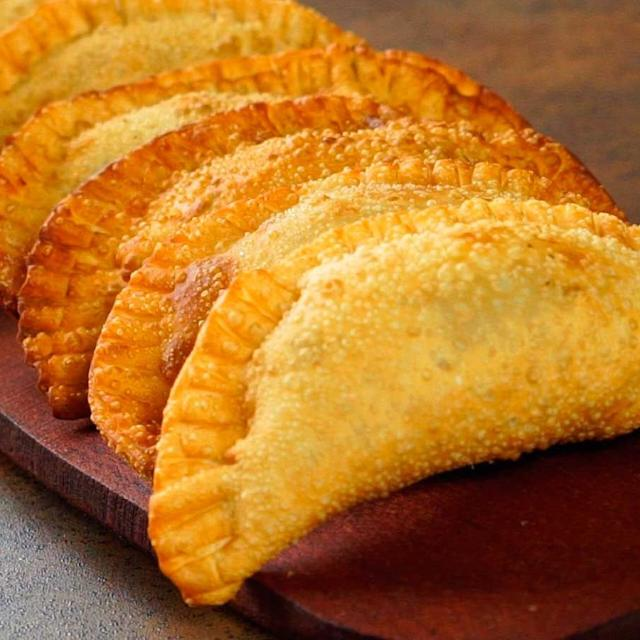
\includegraphics[width=0.95\textwidth]{empanadas} % Logo of the school
\newpage

\tableofcontents
\newpage

\section{Resumen} % Aprox 1/3 de Pagina
El presente informe detalla la planificación inicial y el análisis de factibilidad financiera para el emprendimiento "Las Empanadas Hermanas", un negocio ficticio de venta de empanadas. El proyecto se enmarca en la aplicación de conocimientos de Matemática Financiera. Se seleccionaron tres variedades de empanadas: Pino, Queso Clásica y Camarón Queso, con una producción estimada de 500 unidades de cada una para el primer mes, totalizando 1500 empanadas.

Se realizó una cotización de ingredientes en diversos proveedores, seleccionando las opciones más económicas para elaborar una lista de compras detallada. Con base en esta lista, se simuló una factura de compra, calculando el costo neto de los insumos en \$893.249 y un IVA crédito fiscal de \$169.717.

Posteriormente, se definieron los precios de venta para cada variedad, considerando los costos de producción y un margen de ganancia: \$1.800 para la empanada de Pino, \$2.000 para la de Queso y \$2.500 para la de Camarón Queso (precios finales con IVA). La proyección de ingresos totales por ventas asciende a \$3.150.000, generando un IVA débito fiscal de \$502.940. El IVA a pagar al fisco se estimó en \$333.223.

Finalmente, se calculó una ganancia bruta de \$1.753.811. Esta cifra permite cubrir los costos de producción para el siguiente mes (\$893.249) y deja un saldo a favor de \$860.562 como sueldo para el grupo, cumpliendo con los requisitos de viabilidad inicial del proyecto.
\newpage



\section{Introducción} % Max 1 pagina
El presente informe tiene como objetivo presentar el negocio de empanadas "Las Empanadas Hermanas", un emprendimiento que busca ofrecer empanadas de alta calidad. A través de este documento, se detallarán los aspectos clave del negocio, incluyendo su propuesta de valor, mercado objetivo y proyecciones financieras iniciales correspondientes al primer avance del trabajo de Matemática Financiera. \\

Dentro de las proyecciones financieras, se contempla un análisis de costos y precios para una producción inicial, así como una estimación de las ganancias esperadas. El negocio se enfoca en la producción y venta de tres variedades principales de empanadas: Pino (carne), Queso Clásica, y Camarón Queso, con un énfasis en la calidad de los ingredientes y la satisfacción del cliente. Todo esto se desarrolla sin olvidar el marco legal regulatorio, por lo cual este negocio no será un frente para lavado de activos, evasión de impuestos, generación de facturas ideológicamente falsas, o la venta de drogas ilícitas. \\ % Referencia a Breking Bad y Los Pollos Hermanos. Mantener el toque estudiantil.


\subsection{Objetivos del Negocio:}
\begin{enumerate}
    \item \textbf{Propuesta de Valor Inicial:} Ofrecer tres variedades de empanadas (Pino, Queso, Camarón Queso) de alta calidad, elaboradas con ingredientes frescos, destacando el sabor tradicional.
    \item \textbf{Estimación de Producción y Ventas:} Definir una cantidad inicial de productos a vender para el primer mes (500 unidades por variedad, total 1500 empanadas).
    \item \textbf{Análisis de Costos de Ingredientes:} Cotizar los ingredientes en al menos dos proveedores y seleccionar los más convenientes para elaborar una lista de compras detallada y valorizada.
    \item \textbf{Gestión de IVA en Compras:} Elaborar una factura de compra simulada que refleje el valor neto de los ingredientes, el IVA crédito fiscal y el total pagado.
    \item \textbf{Estrategia de Precios y Proyección de Ingresos:} Definir precios de venta competitivos para cada variedad, que cubran costos y generen ganancia. Calcular el ingreso total neto esperado y el IVA débito fiscal.
    \item \textbf{Cálculo de Obligaciones Tributarias (IVA):} Determinar el monto de IVA a pagar al fisco, resultante de la diferencia entre IVA débito e IVA crédito.
    \item \textbf{Evaluación de Rentabilidad Inicial:} Calcular las ganancias del primer mes y verificar si son suficientes para reinvertir en la producción del mes siguiente y obtener un excedente (sueldo para el grupo).
    \item \textbf{Viabilidad del Negocio (Preliminar):} Evaluar la viabilidad preliminar del negocio basándose en los cálculos financieros del primer mes de operación.

\end{enumerate}

\newpage



\section{Desarrollo} % 2 - 5 paginas
% \subsection{} % This was empty, removed.

\subsection{Tabla de Costos de Ingredientes}

\begin{table}[H] % Using [H] from float package to place it "here"
    \centering
    \begin{tabular}{|| c | c | c | c||} 
        \hline
    \textbf{Distribuidor} & Formato & \textbf{Costo} & \textbf{Costo 100 Unidades} \\ [0.5ex]
        \hline\hline
        \multicolumn{4}{||c||}{\textbf{Masa Prehecha Grande}} \\ [0.5ex] \hline \hline
        El Palacio de las Empanadas & 20 Un & \$4100 & \$20500 \\ \hline
        Masas Mi Tierra & 25 Un & \$8000 & \$31000 \\ \hline
        Alimentos La Kosa & 20 Un & \$4200 & \$21000 \\ [1ex] \hline \hline

        \multicolumn{3}{||c||}{\textbf{Huevos}} & \textbf{Costo por Docena} \\ [0.5ex] \hline \hline
        El Don Huevo & 180 Un & \$39500 & \$2633 \\ \hline
        Huevos La Montaña Pelluhue & 180 Un & \$43990 & \$2932 \\ \hline
        AgricoVial & 180 Un & \$41600 & \$2773 \\ [1ex] \hline \hline

        \multicolumn{3}{||c|}{\textbf{Camaron}} & \textbf{Costo por KG} \\ [0.5ex] \hline \hline
        Distribuidora GK & 10 KG & \$48900 & \$4890 \\ \hline
        Comercial Oceanica & 10 KG & \$55800 & \$5580 \\ \hline
        Del Origen & 10 KG & \$48700 & \$4870 \\ [1ex] \hline \hline

        \multicolumn{3}{||c|}{\textbf{Carne Molida}} & \textbf{Costo por KG} \\ [0.5ex] \hline \hline % Added Costo por KG header for consistency
        Central Mayorista & 500 G & \$2590 & \$5080 \\ \hline 
        Unimarc & 1 KG & \$4990 & \$4990 \\ \hline 
        El Paiquito & 250 G & \$1090 & \$4360 \\ [1ex] \hline \hline


        \multicolumn{3}{||c|}{\textbf{Queso}} & \textbf{Costo por KG} \\ [0.5ex] \hline \hline % Added Costo por KG header
        Distribuidora Santiago & 1 KG & \$9580 & \$9580 \\ \hline
        Distribuidora Nueva de Matte & 1 KG & \$6940 & \$6940 \\ \hline
        Mayorista 10 & 1 KG & \$9160 & \$9160 \\ [1ex] \hline \hline

        \multicolumn{3}{||c|}{\textbf{Cebolla}} & \textbf{Costo por KG} \\ [0.5ex] \hline \hline % Added Costo por KG header
        Santiago Natural Foods & 14 KG & \$10990 & \$785 \\ \hline
        Distribuidora Frest & 10 KG & \$9990 & \$990 \\ \hline
        Lider & 1 KG & \$1195 & \$1195 \\ [1ex] \hline \hline

        \multicolumn{3}{||c|}{\textbf{Aceite}} & \textbf{Costo por Litro} \\ [0.5ex] \hline \hline
        ProsudMarket & 18 L & \$39614 & \$2200.77 \\ \hline
        Central Mayorista & 13.5 L & \$22200 & \$1644.44 \\ \hline
        Distribuidora Sabatini & 5L & \$9296 & \$1859.20 \\ [1ex] \hline \hline

    \end{tabular}
    \caption{Tabla de Costos de Ingredientes por Proveedor}
    \label{tab:costos_ingredientes_proveedor}
\end{table} %Fin Priemra Pagina del Desarrollo
\newpage


\subsection{Cotizaciones de Ingredientes}
    %\subsubsection{Masa Prehecha}
        \begin{figure}[H] % Use [H] or [htbp] for better float placement
            \centering % Center the content of the figure
            \begin{subfigure}{0.4\textwidth}
                \centering
                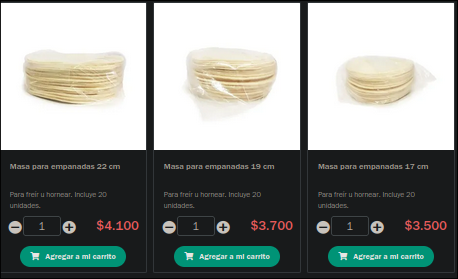
\includegraphics[width=0.9\linewidth]{palaci} % Removed space before ]
                \caption{Palacio de las Empanadas}
                \label{fig:palacio}
            \end{subfigure}
            \hfill % Add some space between subfigures
            \begin{subfigure}{0.4\textwidth}
                \centering
                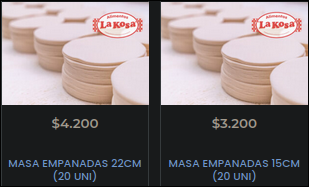
\includegraphics[width=0.9\linewidth]{kosa} % Removed space before ]
                \caption{Alimentos La Kosa}
                \label{fig:kosa}
            \end{subfigure}
            \caption{Cotizaciones de Distribuidores de Masa Prehecha}
            \label{fig:cotizaciones_masas}
        \end{figure} % END OF THIS FIGURE

    %\subsubsection{Huevos}
        \begin{figure}[H] % START A NEW FIGURE
            \centering
            \begin{subfigure}{0.35\textwidth}
                \centering
                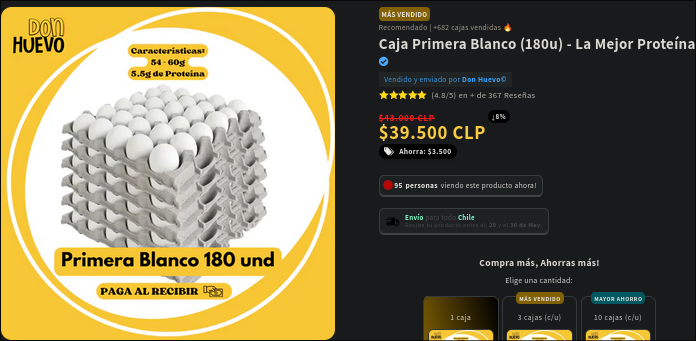
\includegraphics[width=0.9\linewidth]{donhuevo} % Removed space before ]
                \caption{El Don Huevo}
                \label{fig:don_huevo}
            \end{subfigure}
            \hfill
            \begin{subfigure}{0.4\textwidth}
                \centering
                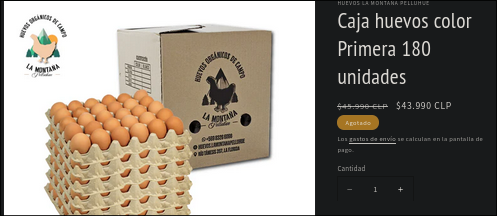
\includegraphics[width=0.9\linewidth]{montan1} % Removed space before ]
                \caption{Huevos La Montaña Pelluhue}
                \label{fig:huevos_montaña}
            \end{subfigure}
            \caption{Cotizaciones de Distribuidores de Huevos}
            \label{fig:cotizaciones_huevos}
        \end{figure} % END OF THIS FIGURE

    %\subsubsection{Camaron}
        \begin{figure}[H] % START A NEW FIGURE
            \centering
            \begin{subfigure}{0.4\textwidth}
                \centering
                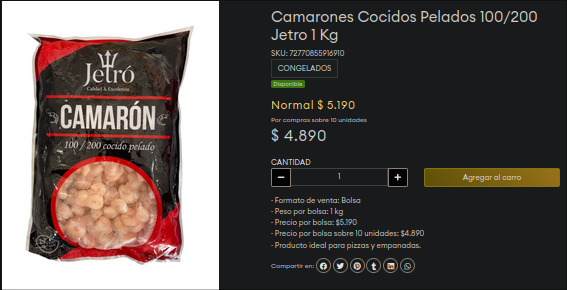
\includegraphics[width=0.9\linewidth]{gk} % Removed space before ]
                \caption{Distribuidora GK}
                \label{fig:distribuidora_gk}
            \end{subfigure}
            \hfill
            \begin{subfigure}{0.35\textwidth}
                \centering
                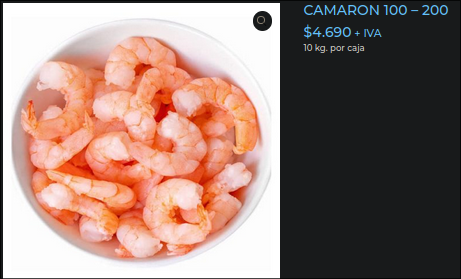
\includegraphics[width=0.9\linewidth]{oceanic} % Removed space before ]
                \caption{Comercial Oceanica}
                \label{fig:comercial_oceanica}
            \end{subfigure}
            \caption{Cotizaciones de Distribuidores de Camarón}
            \label{fig:cotizaciones_camaron}
        \end{figure} % END OF THIS FIGURE
         \newpage 
        % Fin segunda pagina del desarrollo

    %\subsubsection{Carne Molida}
        \begin{figure}[H] % START A NEW FIGURE
            \centering
            \begin{subfigure}{0.45\textwidth}
                \centering
                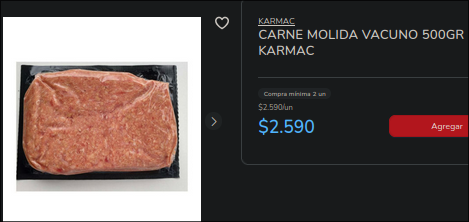
\includegraphics[width=0.9\linewidth]{central} % Removed space before ]
                \caption{Central Mayorista}
                \label{fig:central_mayorista}
            \end{subfigure}
            \hfill
            \begin{subfigure}{0.45\textwidth}
                \centering
                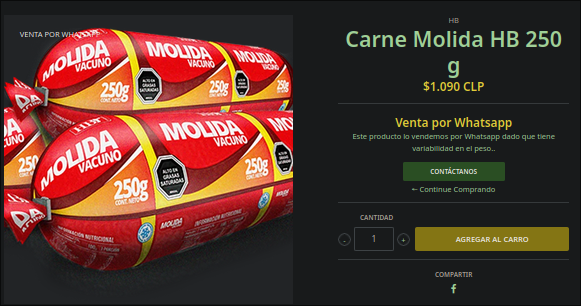
\includegraphics[width=0.9\linewidth]{paiquito} % Removed space before ]
                \caption{Paiquito}
                \label{fig:paiquito} 
            \end{subfigure}
            \caption{Cotizaciones de Distribuidores de Carne Molida}
            \label{fig:cotizaciones_carne_molida}
        \end{figure} % END OF THIS FIGURE

    %\subsubsection{Queso}
        \begin{figure}[H] % START A NEW FIGURE
            \centering
            \begin{subfigure}{0.45\textwidth}
                \centering
                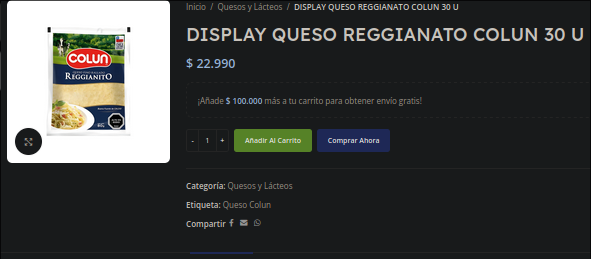
\includegraphics[width=0.9\linewidth]{santiago} % Removed space before ]
                \caption{Distribuidora Santiago}
                \label{fig:distribuidora_santiago}
            \end{subfigure}
            \hfill
            \begin{subfigure}{0.45\textwidth}
                \centering
                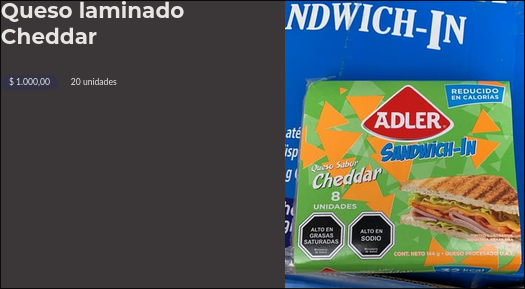
\includegraphics[width=0.9\linewidth]{nueva} % Removed space before ]
                \caption{Distribuidora Nueva de Matte}
                \label{fig:distribuidora_nueva_de_matte}
            \end{subfigure}
            \caption{Cotizaciones de Distribuidores de Queso}
            \label{fig:cotizaciones_queso}
        \end{figure} % END OF THIS FIGURE

    %\subsubsection{Cebolla}
        \begin{figure}[H] % START A NEW FIGURE
            \centering
            \begin{subfigure}{0.4\textwidth}
                \centering
                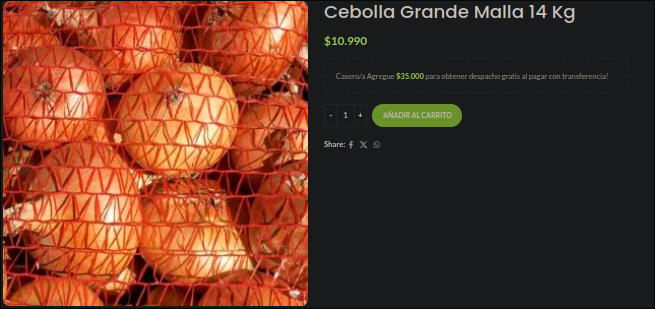
\includegraphics[width=0.9\linewidth]{nat} % Removed space before ]
                \caption{Santiago Natural Foods}
                \label{fig:santiago_natural_foods}
            \end{subfigure}
            \hfill
            \begin{subfigure}{0.45\textwidth}
                \centering
                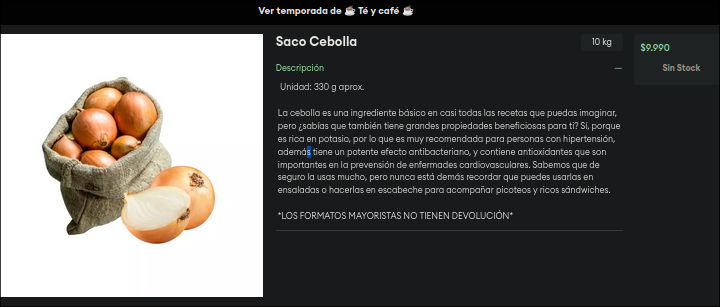
\includegraphics[width=0.9\linewidth]{fres} % Removed space before ]
                \caption{Distribuidora Frest}
                \label{fig:distribuidora_frest}
            \end{subfigure}
            \caption{Cotizaciones de Distribuidores de Cebolla}
            \label{fig:cotizaciones_cebolla}
        \end{figure} % END OF THIS FIGURE

    %\subsubsection{Aceite}
        \begin{figure}[H] % START A NEW FIGURE
            \centering
            \begin{subfigure}{0.45\textwidth}
                \centering
                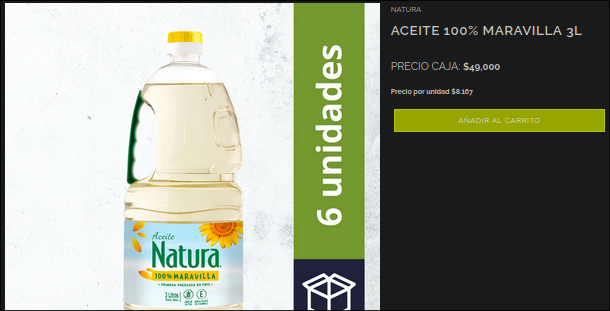
\includegraphics[width=0.9\linewidth]{prosud} % Removed space before ]
                \caption{ProsudMarket}
                \label{fig:prosudmarket}
            \end{subfigure}
            \hfill
            \begin{subfigure}{0.45\textwidth}
                \centering
                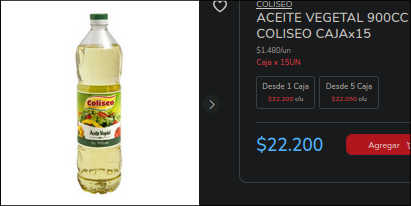
\includegraphics[width=0.9\linewidth]{aceite} % Removed space before ]
                \caption{Central Mayorista}
                \label{fig:central_mayorista_aceite}
            \end{subfigure}
            \caption{Cotizaciones de Distribuidores de Aceite}
            \label{fig:cotizaciones_aceite}
        \end{figure} % END OF THIS FIGURE
        % Fin tercera pagina del desarrollo
        
        \newpage 

    \subsection{Facturas e IVA} 
        \subsubsection{Lista de Compras Detallada y Costos Seleccionados}
        Para la producción inicial de 1500 empanadas (500 de cada variedad: Pino, Queso Clásica, Camarón Queso), se seleccionaron los proveedores con los precios más convenientes para cada ingrediente, según la Tabla \ref{tab:costos_ingredientes_proveedor}. Las cantidades y costos se detallan en la Tabla \ref{tab:lista_compras}.

        \begin{table}[H]
            \centering
            \small % Reduce font size for this table
            \begin{tabular}{|l|l|r|c|r|r|}
                \hline
                \textbf{Ingrediente} & \textbf{Proveedor Elegido} & \textbf{Cantidad} & \textbf{Unidad} & \textbf{Costo Unitario} & \textbf{Costo Total} \\
                \hline
                Masa Prehecha & El Palacio de las Emp. & 1500 & Unidades & \$205 & \$307.500 \\
                Huevos & El Don Huevo & 11 & Docenas & \$2.633 & \$28.963 \\
                Camarón & Del Origen & 20 & KG & \$4.870 & \$97.400 \\
                Carne Molida & El Paiquito & 25 & KG & \$4.360 & \$109.000 \\
                Queso Mantecoso & Dist. Nueva de Matte & 45 & KG & \$6.940 & \$312.300 \\
                Cebolla & Santiago Natural Foods & 15 & KG & \$785 & \$11.775 \\
                Aceite & Central Mayorista & 16 & Litros & \$1.644,44 & \$26.311 \\
                \hline
                \multicolumn{5}{|r|}{\textbf{TOTAL NETO COMPRAS}} & \textbf{\$893.249} \\
                \hline
            \end{tabular}
            \caption{Lista de Compras para 1500 Empanadas.}
            \label{tab:lista_compras}
        \end{table}

        \subsubsection{Factura de Compra Simulada}
        A continuación, se presenta una simulación de la factura de compra de los ingredientes, detallando el valor neto, el IVA (19\%) y el total pagado. Para simplificar, se agrupan todos los insumos en una única factura de un proveedor genérico "Insumos Gourmet Ltda.".

        \begin{table}[H]
            \centering
            \small
            \textbf{FACTURA ELECTRÓNICA N° 001} \\ %\vspace{0.2cm}
            \begin{tabular}{|p{8cm}|p{6cm}|}
                \hline
                \textbf{Proveedor:} & \textbf{Cliente:} \\
                Insumos Gourmet Ltda. & Las Empanadas Hermanas \\
                RUT: 77.777.777-7 & RUT: 78.888.888-8 (Ficticio) \\
                Dirección: Av. Siempre Viva 123, Santiago & Dirección: Taller de Producción, Santiago \\
                Giro: Venta al por mayor de alimentos & Giro: Elaboración y Venta de Comida \\
                \hline
                \textbf{Fecha de Emisión:} 30 de mayo de 2025 & \\
                \hline
            \end{tabular}
            \vspace{0.3cm}
            
            \begin{tabular}{|l|r|r|r|r|}
                \hline
                \textbf{Descripción} & \textbf{Cantidad} & \textbf{P. Unit. Neto} & \textbf{Total Neto} \\
                \hline
                Masa Prehecha Grande (1500 un.) & 1 & \$307.500 & \$307.500 \\
                Huevos (11 docenas) & 1 & \$28.963 & \$28.963 \\
                Camarón Congelado (20 kg) & 1 & \$97.400 & \$97.400 \\
                Carne Molida (25 kg) & 1 & \$109.000 & \$109.000 \\
                Queso Mantecoso (45 kg) & 1 & \$312.300 & \$312.300 \\
                Cebolla (15 kg) & 1 & \$11.775 & \$11.775 \\
                Aceite Vegetal (16 L) & 1 & \$26.311 & \$26.311 \\
                \hline
                \multicolumn{3}{|r|}{\textbf{SUBTOTAL NETO}} & \textbf{\$893.249} \\
                \multicolumn{3}{|r|}{IVA (19\%)} & \$169.717 \\
                \multicolumn{3}{|r|}{\textbf{TOTAL A PAGAR}} & \textbf{\$1.062.966} \\
                \hline
            \end{tabular}
            \caption{Factura de Compra Simulada de Ingredientes.}
            \label{tab:factura_compra}
        \end{table}
    \newpage
    \subsection{Definición de Precios y Proyección de Ingresos}
        \subsubsection{Costos Unitarios y Precios de Venta}
        Se calculó el costo neto de producción por unidad para cada variedad de empanada, considerando los ingredientes y una porción del aceite de fritura. Con base en estos costos y los precios de mercado, se definieron los precios de venta finales (IVA incluido), buscando un margen de ganancia adecuado.

        \begin{table}[H]
            \centering
            \small
            \begin{tabular}{|l|r|r|r|}
                \hline
                \textbf{Variedad Empanada} & \textbf{Costo Prod.} & \textbf{Precio Venta} & \textbf{Precio Venta Final (IVA Inc.)} \\
                \hline
                Pino & \$521,13 & \$1.512,61 & \$1.800 \\
                Queso Clásica & \$637,84 & \$1.680,67 & \$2.000 \\
                Camarón Queso & \$624,44 & \$2.100,84 & \$2.500 \\
                \hline
            \end{tabular}
            \caption{Costos Unitarios y Precios de Venta por Variedad.}
            \label{tab:precios_venta}
        \end{table}
        \textit{Nota: El costo de producción incluye: masa, relleno específico, y una cuota parte del aceite de fritura y preparación.}

        \subsubsection{Proyección de Ingresos y Cálculo de IVA}
        Considerando la venta de 500 unidades de cada variedad, la proyección de ingresos y el cálculo del IVA débito fiscal son los siguientes:

        \textbf{Ingresos por Ventas (Producción de 1500 empanadas):}
        \begin{itemize}
            \item Empanadas de Pino: 500 unidades * \$1.800/unidad = \$900.000
            \item Empanadas de Queso: 500 unidades * \$2.000/unidad = \$1.000.000
            \item Empanadas Camarón Queso: 500 unidades * \$2.500/unidad = \$1.250.000
            \item \textbf{Total Ingresos Brutos (IVA Incluido): \$3.150.000}
        \end{itemize}

        \textbf{Cálculo del IVA:}
        \begin{itemize}
            \item Total Ingresos Netos (Ventas): \$3.150.000 / 1,19 = \$2.647.059 (aprox.)
            \item \textbf{IVA Débito Fiscal (Ventas):} \$2.647.059 * 0,19 = \textbf{\$502.941} (aprox.)
            \item IVA Crédito Fiscal (Compras, Tabla \ref{tab:factura_compra}): \$169.717
            \item \textbf{IVA a Pagar al Fisco:} \$502.941 (Débito) - \$169.717 (Crédito) = \textbf{\$333.224}
        \end{itemize}
        
    \subsubsection{Cálculo de Ganancias y Viabilidad Inicial}
    La ganancia se calcula como la diferencia entre los ingresos netos por ventas y los costos netos de los ingredientes.

    \begin{itemize}
        \item Ingresos Netos Totales por Ventas: \$2.647.059
        \item Costo Neto Total de Ingredientes (Tabla \ref{tab:lista_compras}): \$893.249
        \item \textbf{Ganancia Bruta (Utilidad Bruta):} \$2.647.059 - \$893.249 = \textbf{\$1.753.810}
    \end{itemize}

    Esta ganancia bruta de \$1.753.810 debe ser suficiente para:
    \begin{enumerate}
        \item Cubrir los costos de producción del próximo mes, equivalentes a \$893.249 (suponiendo la misma producción).
        \item Dejar un saldo a favor como sueldo para el grupo.
    \end{enumerate}
    Saldo para sueldo del grupo: \$1.753.810 (Ganancia Bruta) - \$893.249 (Costos Siguiente Mes) = \textbf{\$860.561}.

    Este saldo de \$860.561 se considera aceptable como remuneración para el grupo de 4 estudiantes por el primer mes de operación, cumpliendo así con los requisitos de viabilidad inicial del proyecto.

    \newpage


\section{Conclusiones} % Max 1 pagina
El análisis financiero preliminar para el emprendimiento "Las Empanadas Hermanas" demuestra una viabilidad inicial positiva. La planificación detallada de costos de ingredientes, la selección estratégica de proveedores y la definición de precios de venta competitivos permiten proyectar un escenario favorable para el primer mes de operaciones.

La producción y venta de 1500 empanadas (500 de Pino, 500 de Queso Clásica y 500 de Camarón Queso) generaría ingresos brutos de \$3.150.000. Tras deducir los costos netos de los ingredientes (\$893.249), se obtiene una ganancia bruta de \$1.753.810. Esta cifra es crucial, ya que no solo permite reinvertir en la producción del siguiente ciclo (\$893.249), sino que también arroja un excedente de \$860.561. Este excedente puede ser considerado como el "sueldo" para los integrantes del grupo, satisfaciendo uno de los objetivos clave del proyecto.

Adicionalmente, se ha cumplido con la estimación de las obligaciones tributarias, resultando en un IVA a pagar al fisco de \$333.224, producto de la diferencia entre el IVA débito fiscal (\$502.941) y el IVA crédito fiscal (\$169.717).

Si bien estos cálculos son alentadores, es importante reconocer que se basan en estimaciones y no consideran otros posibles costos operativos (como gas, electricidad, transporte, empaques, permisos, etc.) ni imprevistos. Futuros avances del proyecto deberían incorporar un análisis de costos más exhaustivo para una evaluación de rentabilidad más precisa.

En resumen, el primer avance del proyecto "Las Empanadas Hermanas" cumple con los objetivos planteados, estableciendo una base financiera sólida y demostrando que, bajo las condiciones simuladas, el negocio de venta de empanadas es factible y podría generar beneficios económicos para sus emprendedores.


\end{document}
